% mpc_cuda_report.ja.tex -- 技術報告（日本語）
% コンパイル: uplatex mpc_cuda_report.ja.tex && dvipdfmx mpc_cuda_report.ja
\documentclass[uplatex,dvipdfmx,a4paper,11pt]{jsarticle}
\usepackage{amsmath,amssymb}
\usepackage{booktabs}
\usepackage{array}
\usepackage{listings}
\usepackage{url}
\usepackage[dvipdfmx]{graphicx}
\usepackage[dvipdfmx]{xcolor}
\usepackage[dvipdfmx,colorlinks=true,linkcolor=blue,citecolor=blue,urlcolor=blue]{hyperref}
\usepackage{pxjahyper}

\lstset{
  basicstyle=\ttfamily\small,
  frame=single,
  breaklines=true,
  columns=fullflexible,
  keepspaces=true,
  showstringspaces=false,
  xleftmargin=1.5em,
  framexleftmargin=1.5em,
}
\newcommand{\code}[1]{\texttt{#1}}

\title{mpc\_cuda: GMP/MPFR/MPC の CUDA 移植\\
{\large ---- 作成手順・実装上の困難・性能評価 ----}}
\author{tkouya}
\date{\today}

\begin{document}
\maketitle

\begin{abstract}
本報告は，任意精度演算ライブラリ群 GNU MP (GMP) / MPFR / MPC を
NVIDIA GPU の CUDA カーネル内部で動作させたライブラリ \textbf{mpc\_cuda} の
作成手順，移植過程で直面した実装上の困難とその解決，および基本線形計算と
初等関数の性能評価をまとめたものである。さらに，コンパイル時に精度を固定する
レジスタ常駐型の高速パス \code{cu\_freal<PB>}/\code{cu\_fcomplex<PB>} を新設し，
精度 128--8192 ビットでの GPU・CPU 性能のクロスオーバーを定量的に示す。
主対象ハードウェアは NVIDIA GB10（compute capability 12.1，\code{sm\_121}，CUDA 13）であり，
さらにランタイム精度デモを NVIDIA H100 NVL（compute capability 9.0，\code{sm\_90}）と
クロス比較する。全結果はホストの MPFR/MPC とビット一致（または初等関数で $\le 1$ ULP）である。
\end{abstract}

\tableofcontents
\bigskip

%======================================================================
\section{はじめに}
\label{sec:intro}

GPU 上で任意精度演算を行いたいという要求は，悪条件問題の数値線形代数や
高精度シミュレーションなどで根強い。既存の GPU 向け多倍長ライブラリ
（例：CUMP は GMP の \code{mpf} を移植）は存在するが，丸めの規約が緩く，
複素数や初等関数を欠くものが多い。本プロジェクトの目標は，
\textbf{正しく丸められる MPFR の実数意味論}と
\textbf{その上の複素数層 MPC}を，可能な限り\textbf{忠実に}（再実装ではなく
上流ソースの移植として）CUDA カーネル内で動かすことである。
具体的な到達目標は，\code{y = a\,x + y}（AXPY）を実数（MPFR）・複素（MPC）の
両方で GPU 上で実行し，CPU 版とビット一致させ，かつ十分に高速化することであった。

本報告の構成は次の通りである。
第\ref{sec:procedure}節で全体設計と作成手順（変換スクリプト方式と層別の段階）を述べ，
第\ref{sec:difficulties}節で移植上の困難と解決を詳述する。
第\ref{sec:fixed}節でコンパイル時固定精度の高速パスを，
第\ref{sec:perf}節で性能評価（AXPY，基本線形計算，初等関数，精度スイープ）を示し，
第\ref{sec:conclusion}節でまとめる。

%======================================================================
\section{全体設計と作成手順}
\label{sec:procedure}

\subsection{出発点となる上流ソース}

移植の土台として，GMP のサブセット実装である \textbf{mini-gmp}
（\code{gmp-6.3.0/mini-gmp}）を採用した。mini-gmp は単一の C ソースで
\code{mpz}（多倍長整数）と \code{mpn}（低レベルリム列）の主要部を提供する。
MPFR-4.2.2 は \code{--with-mini-gmp} オプションで mini-gmp 上にビルドでき，
不足する \code{mpn} ルーチン（\code{mpn\_divrem} 等）は MPFR 同梱の
\code{mpfr-mini-gmp.c} が補う。すなわち\textbf{フル GMP の内部実装を必要としない}。
MPC-1.4.1 は MPFR の上の薄い複素層であり，同じ土台に載る。

\subsection{変換スクリプト方式}

上流を手作業でフォークすると上流更新の取り込みが困難になる。そこで本プロジェクトでは
\textbf{再実行可能な変換スクリプト}（\code{tools/cudafy\_*.py}）で
デバイス適応を行う方針を採った。

\begin{itemize}
\item \code{tools/cudafy\_minigmp.py}: pristine な \code{mini-gmp.\{c,h\}} を読み，
      デバイス到達関数に \code{\_\_host\_\_ \_\_device\_\_} を付与した
      \code{include/mpc\_cuda/cuda\_minigmp.h} と \code{src/cuda\_minigmp.cu} を生成する。
      ホスト専用関数（stdio/realloc/ctype を使うもの）は字句走査で自動判定する。
\item \code{tools/cudafy\_mpfr.py}: MPFR の 263 個のソースに同様の適応を施す。
\item \code{tools/cudafy\_mpc.py}: MPC の 90 個のソースに適応を施す（MPFR 用の機構を再利用）。
\end{itemize}

これにより上流の構造を保ったまま，スクリプトの再実行で更新を再適用できる。

\subsection{層別の段階}

開発は次の 4 段階（＋ 2b）で進めた。各段階はホスト版とビット一致を確認しながら積み上げた。

\begin{table}[h]
\centering
\caption{層別の開発段階}
\begin{tabular}{clp{7.5cm}}
\toprule
段階 & 層 & 内容 \\
\midrule
1  & mini-gmp & \code{mpz}/\code{mpn} をデバイスで動作。add/sub/mul/tdiv\_qr/pow\_ui/get\_str をホストとビット一致（256 スレッド）。\\
2  & MPFR（忠実移植）& 実 \code{mpfr-4.2.2} の init2/set/mul/add/get\_d がカーネル内で動作。\\
2b & MPFR 超越関数 & pi/exp/log/sin/cos/atan/sqrt が動作（後述の \code{mpfr\_div} 代替が必要）。\\
3  & MPC（複素）& 実 \code{mpc-1.4.1} の init2/set\_d\_d/mul/add が動作。\\
4  & AXPY デモ・ベンチ & 実・複素の AXPY を GPU/CPU で時間・精度比較。\\
\bottomrule
\end{tabular}
\end{table}

%======================================================================
\section{実装上の困難とその解決}
\label{sec:difficulties}

「コンパイルが通る」ことと「デバイスで正しく動く」ことは別問題である。
本節では移植の核心となった困難を分類して述べる。

\subsection{コンパイルを通すための適応}

\begin{enumerate}
\item \textbf{C11 \code{\_Noreturn}}：nvcc の C++ フロントエンドが \code{\_Noreturn} を
      拒否する。ホスト版にある \code{-DMPFR\_HAVE\_NORETURN} を\textbf{外す}。
\item \textbf{インラインアセンブリ}：\code{mpfr-longlong.h} の x86\_64 用 \code{umul\_ppmm}
      等はデバイスで無効。\code{-DNO\_ASM} で移植版 C フォールバックを選択する。
\item \textbf{realloc の不在}：CUDA デバイスコードに \code{realloc} が無い。
      malloc+memcpy+free で擬似的に実装する（\code{mg\_cuda\_realloc}）。
\item \textbf{C99 \code{\_Complex}}：デバイスコードに \code{\_Complex} が無い。
      MPC の \code{mpc.h} の \code{\#if 1}（\code{\_MPC\_HAVE\_COMPLEX\_H} 定義）を
      \code{\#if 0} に変え，\code{mpc\_set\_dc}/\code{get\_dc} を無効化する。
\item \textbf{\code{gmp.h} シム}：MPC の \code{mpc.h} は \code{gmp.h} を \code{\#include} する。
      mini-gmp を指す \code{gmp.h} シムを生成し，mini-gmp に無い
      \code{gmp\_randstate\_t}/\code{mpf\_t}/\code{mpq\_t} の最小スタブを宣言してプロトタイプを通す。
\item \textbf{トークン貼り付け}：MPC の \code{set\_x.c}/\code{set\_x\_x.c} は
      \code{mpfr\_set\_\#\#type} で全 setter を 1 つの翻訳単位に展開し，
      mini-gmp に無い \code{mpfr\_set\_f}/\code{\_q} を巻き込む。
      これらにトラップするデバイススタブを注入してコンパイルを通す（未使用なら呼ばれない）。
\end{enumerate}

\subsection{デバイスで正しく動かすための適応}

ここからが本質的に難しい部分である。コンパイルが通っても，
ホスト前提のグローバル状態・関数ポインタ・最適化が
デバイスで誤動作する。

\begin{enumerate}
\item \textbf{ルックアップテーブル}：\code{invert\_limb\_table} や \code{\_\_clz\_tab} 等の
      ファイルスコープ \code{static const} 配列はデバイスから参照できない。
      \code{MPFR\_RODATA} タグ（デバイスパスで \code{\_\_device\_\_}，ホストパスで空）を付け，
      1 つの定義で両パスを賄う。
\item \textbf{グローバル状態}：\code{\_\_gmpfr\_emin}/\code{emax}/\code{flags} や
      既定精度・丸めは \code{\_\_device\_\_ \_\_managed\_\_}（ホスト・デバイス共有）にする。
\item \textbf{assert/abort}：\code{mpfr\_assert\_fail}（fprintf+abort）や \code{gmp\_die} は
      デバイスで \code{\_\_trap()} に置換する。
\item \textbf{\code{\_\_builtin\_unreachable} の誤コンパイル}：
      \code{MPFR\_HAVE\_BUILTIN\_UNREACHABLE} を有効にすると，その
      \code{\_\_builtin\_constant\_p}/\code{\_\_builtin\_unreachable} 経路が
      \code{MPFR\_ASSERTN} をデバイスで\textbf{誤コンパイル}し，
      本来真の表明が発火した。この define を\textbf{外す}と正常化する。
\item \textbf{確保ルーチンの経路}（特に厄介）：mini-gmp モードの
      \code{mpfr\_allocate\_func}（\code{mpfr-gmp.c}）は
      \code{mp\_get\_memory\_functions()} 経由で mini-gmp の確保フックを取得するが，
      これは\textbf{ホストの関数ポインタ}である。デバイスから呼ぶと
      ゴミ（サイズをそのまま返す \code{0x28} 等）を返した。
      \code{\_\_CUDA\_ARCH\_\_} 下で \code{mpfr\_allocate/reallocate/free\_func} が
      デバイスヒープ（\code{malloc}/\code{free}）を直接呼ぶようにパッチした。
\item \textbf{定数キャッシュ}：\code{mpfr\_const\_pi/log2/euler/catalan} は
      計算関数\textbf{ポインタ}（ホストアドレス）を静的初期化で持ち，共有可変グローバルに
      メモ化する。デバイスでは違法命令・データ競合になる。
      これらを \code{MPFR\_SAVE\_EXPO} を伴うキャッシュレスのラッパ
      \code{mpfr\_const\_*\_cuda} に振り替え，\code{*\_internal} を直接呼ぶ
      （\code{SAVE\_EXPO} を省くと値が誤る）。
\end{enumerate}

\subsection{最大の難関：デバイスでの \code{mpfr\_div} 誤コンパイル}

最も根深い問題は，\textbf{\code{mpfr\_div} の汎用経路（精度 $\ge 3$ リム）が
デバイスで誤コンパイルされ \code{inf}/ゴミを返す}ことであった
（\textbf{同一コードがホストでは正しい}）。これは波及し，
\code{const\_pi}/\code{const\_log2} が内部で除算するため誤値・クラッシュを生み，
\code{log, sin, cos, atan, large exp} を一括して阻んだ
（以前観測した \code{const\_pi} 由来の \code{mpn\_sqrtrem p[n-1]==0} 表明は，
壊れた商が AGM の \code{mpfr\_sqrt} に非正規値を供給した\textbf{下流の症状}であった）。

徹底的な二分切り分けで全ての下位プリミティブが\textbf{単体ではデバイスで正しい}ことを確認した
（\code{mpn\_divrem\_1}, \code{mpn\_divrem}, mini-gmp の \code{mpz} 除算,
\code{count\_leading\_zeros}, \code{udiv\_qrnnd}, \code{MPFR\_TMP}）。
\code{-O0}/\code{-G} でも直らず，誤コンパイルされる構文の文単位の特定も
（計装書き込みが呼び出し前後で並べ替え・脱落して）困難であった。
そこで nvcc のコード生成問題を追うのをやめ，
\textbf{\code{mpz} プリミティブのみで構成した自己完結・正しく丸められる
\code{mpfr\_div}}（\code{mpfr\_div\_cuda}）を代替実装した。
被除数・除数の仮数を \code{mpz} に組み立て，ガードビット付きで 1 回 \code{mpz\_tdiv\_qr} を行い，
round/sticky と剰余から RNDN/Z/U/D/A を丸め，指数を設定して \code{mpfr\_check\_range} する。
公開 \code{mpfr\_div} は \code{\#ifdef \_\_CUDA\_ARCH\_\_} でデバイスのみこれを呼ぶ。
結果は host \code{mpfr\_div} とビット一致（7/2, 1/3, 7/1e9+7, 355/113@500b, 2/7@1024b で検証）し，
これにより全超越関数がデバイスで動作した（\code{make test-mpfr-trans}: 128/128 スレッド一致）。

\subsection{スタック・アリーナ・並列度}

\begin{enumerate}
\item \textbf{スタックオーバーフロー}：\code{mpc\_mul} $\to$ \code{mpfr\_fmms} $\to$
      \code{mpfr\_sub} $\to$ \code{mpfr\_sub1} のような深い呼び出し連鎖は，
      MPFR の大きなスタックフレームと相まって既定の約 1\,KB の CUDA スレッドスタックを溢れさせる。
      \code{cudaDeviceSetLimit(cudaLimitStackSize, 128\,KB)} で引き上げる。
\item \textbf{確保チャーン}：要素ごとに多数のデバイス \code{malloc}/\code{free} が走ると
      その確保処理が支配的になる（アリーナ導入前は実 AXPY が 0.9 倍）。
      \textbf{スレッド毎のバンプアリーナ}（固定スラブを bump 確保，free は no-op，
      作業項目ごとに reset）でこのチャーンを除去した。
\item \textbf{並列度不足}：深い連鎖の中間リムは（グローバルメモリの）アリーナスラブに置かれるため，
      メモリレイテンシを隠すには多数の常駐ワープが要る。小さな起動では飢餓状態になり
      （MPC は N=1024 で 0.7 倍）。\textbf{固定プールの $\sim$8--16K 常駐スレッドが
      ベクトルをグリッドストライドする}構成でレイテンシを隠し，約 40 倍を得た。
\end{enumerate}

\subsection{共存：cu\_ 名前空間と umbrella ヘッダ}

CPU 版の本物の \code{libgmp}/\code{libmpfr}/\code{libmpc} と同一バイナリに同居させるため，
全ての公開シンボルを \code{cu\_} 名前空間へ機械的に改名した
（\code{mpfr\_mul}$\to$\code{cu\_mpfr\_mul} など，\code{tools/cu\_prefix.py}）。
さらに型名・enum 定数・公開マクロ・include ガードもシステムヘッダと衝突するため，
それらも \code{cu\_}/\code{CU\_} で名前空間化した単一インクルードの
\textbf{umbrella ヘッダ}（\code{mpc\_cuda.cuh}）を \code{tools/make\_umbrella.py} で生成した。
これにより \code{\#include "mpc\_cuda.cuh"} 一行で，システムの
\code{<gmp.h>/<mpfr.h>/<mpc.h>} と\textbf{同一翻訳単位}に置いても衝突しない。

\subsection{その他のバグと教訓}

\begin{itemize}
\item \textbf{\code{mul.c} のインライン PTX バグ}：\code{src/mpfr\_cuda/mul.c} に
      手書き PTX の \code{add\_ssaaaa(\dots, 0, t)} があり，整数リテラル \code{0}（4 バイト）を
      64 ビット制約 \code{"l"} に渡してコンパイルエラーになっていた。
      \code{(mp\_limb\_t)\,0} へキャストして解消。これが \code{mul.o}
      （\code{cu\_mpfr\_mul}）の欠落を招き，cu\_mpfr/cu\_mpc 系の再リンクを一時的に阻んでいた。
\item \textbf{\code{cudaLimitStackSize} の戻り値}：GB10 では \code{cudaLimitStackSize} に
      設定可能な上限（数百 KB）があり，512\,KB の要求は \code{cudaErrorInvalidValue} で
      \textbf{拒否}される。戻り値を検査しないとスタックは既定の 1\,KB のままとなり，
      深い cu\_mpc 連鎖がスタックオーバーフロー（``illegal memory access'' として観測）する。
      128\,KB は受理され十分である。\textbf{\code{cudaDeviceSetLimit} は必ず戻り値を検査せよ}。
\end{itemize}

%======================================================================
\section{コンパイル時固定精度の高速パス}
\label{sec:fixed}

ランタイム精度の MPFR/MPC 移植とは別に，\textbf{精度をコンパイル時テンプレート引数で
固定}することで仮数をレジスタに常駐させる高速パスを新設した。

\subsection{設計}

\code{cu\_fp::cu\_freal<PB>}（実数）と \code{cu\_fp::cu\_fcomplex<PB>}（複素）は
ヘッダオンリーのテンプレートである。\code{PB} は仮数ビット幅で\textbf{32 の倍数}
（32, 64, 96, \dots, 256, 512, 1024, \dots）を取れる。
仮数は $\lceil PB/64\rceil$ 個の 64 ビットリム配列で保持し，
精度がコンパイル時定数のため schoolbook 乗算が完全アンロールされ，
\code{ptxas} がローカル配列をレジスタに昇格する（global メモリのアリーナ往復が無い）。
丸めは単一の \code{finalize()} ヘルパに集約し，sub-limb 境界
（\code{SB}$\in\{0,32\}$）を含む任意精度を統一処理する。
演算は \code{+ - *} 演算子と \code{from\_double}/\code{(double)} 変換を備える。
実数の mul/add/sub は MPFR の RNDN と\textbf{ビット一致}し（\code{PB}=32--2048 で検証），
複素乗算は各成分を正しく丸めた実部 $\circ(a_r b_r - a_i b_i)$，
虚部 $\circ(a_r b_i + a_i b_r)$ を\textbf{完全な 2N リム積から 1 回だけ丸めて}
求め，MPC の \code{MPC\_RNDNN} とビット一致する。

\subsection{初等関数}

\code{cu\_fmath.cuh}/\code{cu\_fcmath.cuh} は固定精度の初等関数を提供する：
実数 \code{cu\_\{sqrt,cbrt,exp,expm1,log,log1p,sin,cos,tan,atan,sinh,cosh,asin,acos,atanh,pow\}}，
複素 \code{cu\_\{cexp,clog,csqrt,csin,ccos,ctan,csinh,ccosh\}}。
方針は\textbf{ガードビット付き高精度近似}であり，作業精度 \code{PB+128} ビットで
Newton 反復（div/sqrt/cbrt）と引数簡約級数（exp/log/三角/双曲）を計算し
\code{PB} に丸める。\textbf{正しい丸めは追求しない}（Table Maker's Dilemma の困難ケースは
非有界な Ziv ループを要し，固定精度・レジスタ常駐と相容れない）。
MPFR/MPC との一致は $\le 1$ ULP，検証範囲（PB=64--1024）では経験的に 0 ULP であった。
特殊関数（gamma, zeta, erf, Bessel, Ai）は今後の課題として除外した。

%======================================================================
\section{性能評価}
\label{sec:perf}

主対象は NVIDIA GB10（compute capability 12.1，CUDA 13，\code{-fmad=false}）であり，
比較対象として NVIDIA H100 NVL（compute capability 9.0，\code{sm\_90}）の結果を
各項目で\textbf{並列に併記}する。特記なき限り精度は 1024 ビット，
全結果はホストとビット一致（初等関数は $\le 1$ ULP）である。
2 台のホスト CPU が異なる（GB10 の Grace ARM と H100 機の x86）ため，
GPU 同士の公平な指標は\textbf{GPU 時間 [ms]}であり，GPU 対 CPU 速度比は
各々自ホストを基準とする参考値として併記する。各 GPU を直接対比する
クロスプラットフォーム比較（AXPY・線形計算・初等関数・精度スイープを通した総括）は，
\textbf{本節の最後}（第\ref{sec:platform}節）にまとめる。

\subsection{AXPY（実数・複素）}

ランタイム精度 MPFR/MPC 移植の AXPY \code{y = a\,x + y}（N=16384，1024 ビット）を
GPU と CPU（本ライブラリのホスト経路）で比較した。同じデモを H100 でも実行し，
GB10 と並べて表\ref{tab:axpy}に示す（GPU 時間で H100 が約 4 倍速い）。

\begin{table}[h]
\centering
\caption{ランタイム精度 AXPY（N=16384，1024 ビット，全ビット一致）。
速度比は各々自ホスト CPU 基準（GB10：Grace ARM，H100：x86）。}
\label{tab:axpy}
\begin{tabular}{lrrr@{\hskip 2em}rr}
\toprule
 & \multicolumn{3}{c}{GB10（sm\_121）} & \multicolumn{2}{c}{H100（sm\_90）}\\
\cmidrule(r){2-4}\cmidrule(l){5-6}
デモ & GPU & CPU & 速度比 & GPU & 速度比 \\
\midrule
MPFR 実数 & 1.17\,ms & 48.2\,ms  & 41.3$\times$ & 0.295\,ms & 143$\times$ \\
MPC  複素 & 4.81\,ms & 191.7\,ms & 39.9$\times$ & 1.037\,ms & 160$\times$ \\
\bottomrule
\end{tabular}
\end{table}

高速化にはバンプアリーナ（確保チャーン除去）と十分な常駐スレッド数
（メモリレイテンシ隠蔽）の双方が不可欠であった（第\ref{sec:difficulties}節）。

\subsection{基本線形計算（行列ベクトル積・行列積）}

行列ベクトル積 \code{y=A\(\cdot\)x} と行列積 \code{C=A\(\cdot\)B} を実・複素で実装した
（表\ref{tab:linalg}）。内積のアキュムレータ・スクラッチを\textbf{スタック常駐}
（\code{MPFR\_DECL\_INIT}／複素は \code{mpfr\_custom\_init\_set} ベースの \code{MPC\_DECL\_INIT}）
とし，アリーナは 1 回の積和ぶんのみ保持して内側反復ごとに reset する。
出力要素をグリッドストライドするため $O(N^2)$ の行列積がデバイスを飽和させ，
行列積では 100 倍超を得た。全結果ビット一致。同じカーネルを H100 でも実行し，
GB10 と並べて表\ref{tab:linalg}に示す。H100 は飽和する行列積で速い一方，
小 $N$ の行列ベクトル積では占有率不足で GB10 に劣る（詳細は第\ref{sec:platform}節）。

\begin{table}[h]
\centering
\caption{多倍長線形計算（1024 ビット，全ビット一致）。速度比は各々自ホスト CPU 基準。}
\label{tab:linalg}
\begin{tabular}{lrrrr@{\hskip 2em}rr}
\toprule
 & & \multicolumn{3}{c}{GB10（sm\_121）} & \multicolumn{2}{c}{H100（sm\_90）}\\
\cmidrule(r){3-5}\cmidrule(l){6-7}
カーネル & $N$ & GPU & CPU & 速度比 & GPU & 速度比 \\
\midrule
MPFR 行列ベクトル積 & 256 & 11.3\,ms & 177\,ms  & 15.6$\times$           & 15.80\,ms & 9.2$\times$ \\
MPFR 行列積        & 96  & 23.0\,ms & 2.41\,s  & \textbf{105$\times$}  & 12.00\,ms & \textbf{175$\times$} \\
MPC  行列ベクトル積 & 128 & 24.4\,ms & 179\,ms  & 7.3$\times$           & 29.68\,ms & 5.2$\times$ \\
MPC  行列積        & 64  & 27.9\,ms & 2.88\,s  & \textbf{103$\times$}  & 15.63\,ms & \textbf{155$\times$} \\
\bottomrule
\end{tabular}
\end{table}

\subsection{初等関数}

N=4096 入力に対し関数群を評価した（GPU vs CPU，全関数ビット一致）。
\begin{itemize}
\item \textbf{MPFR}：\code{sqrt cbrt exp expm1 log log1p sin cos tan atan sinh cosh}
      $\Rightarrow$ GPU で \textbf{42--77$\times$}。
\item \textbf{MPC}：\code{sqr sqrt exp log sin cos tan sinh cosh asin acos atan}
      $\Rightarrow$ GPU で \textbf{22--63$\times$}。
\end{itemize}

関数別の内訳を表\ref{tab:elemh100}・図\ref{fig:elemh100}に並列に示す。
\textbf{H100 は関数別の実測値}（GPU vs 自ホスト CPU）を掲げ，
\textbf{GB10 は同一関数群の範囲}（上記の MPFR：42--77$\times$，MPC：22--63$\times$）を
\textbf{灰色帯として併記}する（GB10 の関数別計測は本機では再取得できないため範囲で示す）。
両者は同形でより広い分布を示し，軽量カーネル
（\code{sqrt}・\code{cbrt}・\code{sqr}）は GPU 側が短時間で済む一方ホスト MPFR/MPC は
セットアップ支配のため 170--217$\times$ に達し，多段 AGM を要する重いカーネル
（\code{log}，複素 \code{asin}/\code{acos}）が下端となる。なお GB10 と H100 の速度比は
それぞれ自機の CPU を基準とするため比として直接の比較はできない。

\begin{table}[h]
\centering
\caption{初等・超越関数の GPU 速度比（N=4096，1024 ビット，全ビット一致）。
H100 は関数別の実測，GB10 は同一関数群の範囲（MPFR：42--77$\times$，MPC：22--63$\times$）を併記。}
\label{tab:elemh100}
\footnotesize
\begin{tabular}{lrrr@{\hskip 2em}lrrr}
\toprule
\multicolumn{4}{c}{MPFR（実数）} & \multicolumn{4}{c}{MPC（複素）}\\
\cmidrule(r){1-4}\cmidrule(l){5-8}
関数 & GPU & CPU & 速度比 & 関数 & GPU & CPU & 速度比\\
\midrule
sqrt  & 0.86  & 185.9  & 217$\times$ & sqr  & 0.24  & 42.6    & 180$\times$\\
cbrt  & 3.51  & 597.7  & 170$\times$ & sqrt & 2.93  & 362.6   & 124$\times$\\
exp   & 10.60 & 1271.3 & 120$\times$ & exp  & 23.71 & 3255.8  & 137$\times$\\
expm1 & 9.69  & 1305.7 & 135$\times$ & log  & 77.46 & 6378.9  & 82$\times$\\
log   & 39.71 & 4189.5 & 105$\times$ & sin  & 24.79 & 1398.0  & 56$\times$\\
log1p & 25.99 & 3510.6 & 135$\times$ & cos  & 24.75 & 1396.7  & 56$\times$\\
sin   & 3.14  & 362.1  & 115$\times$ & tan  & 36.80 & 1583.7  & 43$\times$\\
cos   & 2.05  & 219.4  & 107$\times$ & sinh & 24.66 & 1422.3  & 58$\times$\\
tan   & 3.37  & 380.3  & 113$\times$ & cosh & 24.61 & 1420.5  & 58$\times$\\
atan  & 21.75 & 1834.1 & 84$\times$  & asin & 87.69 & 6886.2  & 79$\times$\\
sinh  & 20.75 & 957.1  & 46$\times$  & acos & 94.98 & 7511.9  & 79$\times$\\
cosh  & 14.32 & 936.4  & 65$\times$  & atan & 121.12& 11179.5 & 92$\times$\\
\bottomrule
\end{tabular}\\[2pt]
\footnotesize 時間は ms。参考：GB10（同一関数群）の速度比範囲は
MPFR：42--77$\times$，MPC：22--63$\times$（関数別の内訳は灰色帯として図\ref{fig:elemh100}に併記）。
\end{table}

\begin{figure}[h]
\centering
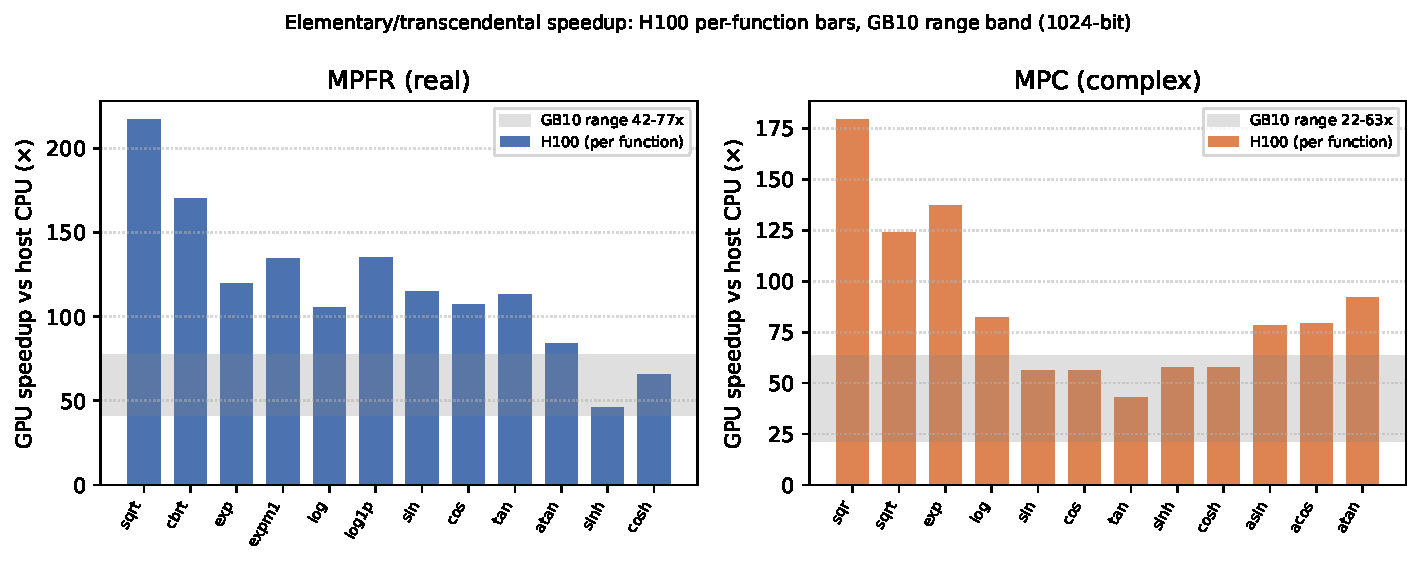
\includegraphics[width=0.95\textwidth]{figures/fig_h100_elem.pdf}
\caption{初等・超越関数の GPU 速度比（対 自ホスト CPU）。
棒＝H100 の関数別実測，灰色帯＝GB10 の範囲（MPFR：42--77$\times$，MPC：22--63$\times$）。
左：MPFR（実数），右：MPC（複素）。1024 ビット，全ビット一致。}
\label{fig:elemh100}
\end{figure}

\subsection{固定精度高速パスと精度スイープ}
\label{sec:sweep}

固定精度パスはランタイム精度パスより大幅に速い。1024 ビット AXPY（N=$2^{20}$）で
\code{cu\_freal} は既存の cu\_mpfr-GPU 経路の \textbf{142 倍}，system CPU MPFR の
\textbf{352 倍}であった（いずれもビット一致）。

精度依存を明らかにするため，AXPY を掃引した（\code{make bench3}）。GB10 は
128--8192 ビット（表\ref{tab:bench3}），H100 は固定・ランタイム・CPU の各経路が
\textbf{完全に交差するまで 128--65536 ビットへ延長}した（表\ref{tab:bench3h100}）。
GB10 と H100 を重ねた時間・速度比を図\ref{fig:real}（実数）・図\ref{fig:complex}（複素）・
図\ref{fig:speedup}（速度比）に示す（実線＝H100，破線＝GB10）。

GB10 では \code{cu\_freal} の時間は 1024 ビットまでほぼ一定（完全レジスタ常駐），
\textbf{2048 ビットで約 7 倍に跳ね上がる}（仮数 $N=32$ リムでレジスタに収まらず
ローカルメモリへスピルする境界），8192 ビットで CPU 1 コアと同等になる。
複素も同形でより大きなリードを示す（1024 ビットで cu\_mpc 比 約 48$\times$，CPU 比 約 107$\times$）。

\begin{table}[h]
\centering
\caption{固定精度パスの精度スイープ（AXPY，N=4096，GB10，全ビット一致）}
\label{tab:bench3}
\begin{tabular}{rrrrrr}
\toprule
ビット & \code{cu\_freal} & \code{cu\_mpfr} & CPU & freal/cu\_mpfr & freal/CPU \\
\midrule
128  & 0.005 & 0.050 & 0.190 & 10.2$\times$ & 38.5$\times$ \\
256  & 0.005 & 0.088 & 0.222 & 19.6$\times$ & 49.1$\times$ \\
512  & 0.006 & 0.174 & 0.320 & 29.5$\times$ & 54.1$\times$ \\
1024 & 0.008 & 0.388 & 0.677 & 47.4$\times$ & \textbf{82.6$\times$} \\
2048 & 0.056 & 0.506 & 0.322 & 9.0$\times$  & 5.7$\times$ \\
4096 & 0.184 & 0.996 & 0.473 & 5.4$\times$  & 2.6$\times$ \\
8192 & 0.823 & 1.989 & 0.814 & 2.4$\times$  & \textbf{1.0$\times$} \\
\bottomrule
\end{tabular}\\[2pt]
\footnotesize 時間は ms（8 回平均）。
\end{table}

\begin{figure}[h]
\centering
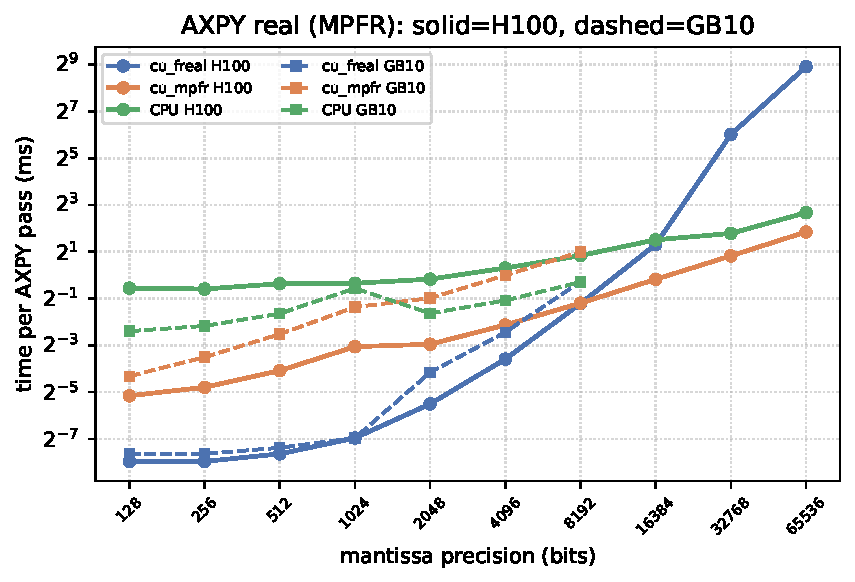
\includegraphics[width=0.95\textwidth]{figures/fig_bench3_real.pdf}
\caption{実数 AXPY の時間 vs 精度（両対数）。実線＝H100（65536 ビットまで），
破線＝GB10（8192 ビットまで）。青＝\code{cu\_freal}，橙＝\code{cu\_mpfr}，緑＝CPU。
固定精度は 1024 ビットまで一定で，2048 ビットでスピルにより跳ね上がり，H100 では
8192 ビットで cu\_mpfr と，16384 ビットで CPU と交差し，以降急激に最悪化する。}
\label{fig:real}
\end{figure}

\begin{figure}[h]
\centering
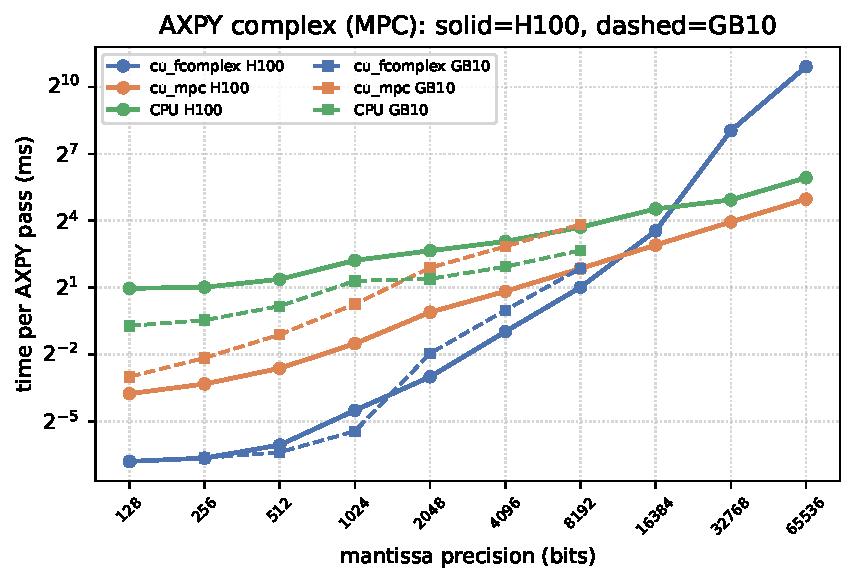
\includegraphics[width=0.95\textwidth]{figures/fig_bench3_complex.pdf}
\caption{複素 AXPY の時間 vs 精度（両対数）。系列は図\ref{fig:real}と同様。実数と同形で
固定精度のリードはより大きいが，H100 では \code{cu\_fcomplex} が 16384 ビットで cu\_mpc と，
32768 ビット手前で CPU と交差する。}
\label{fig:complex}
\end{figure}

\begin{figure}[h]
\centering
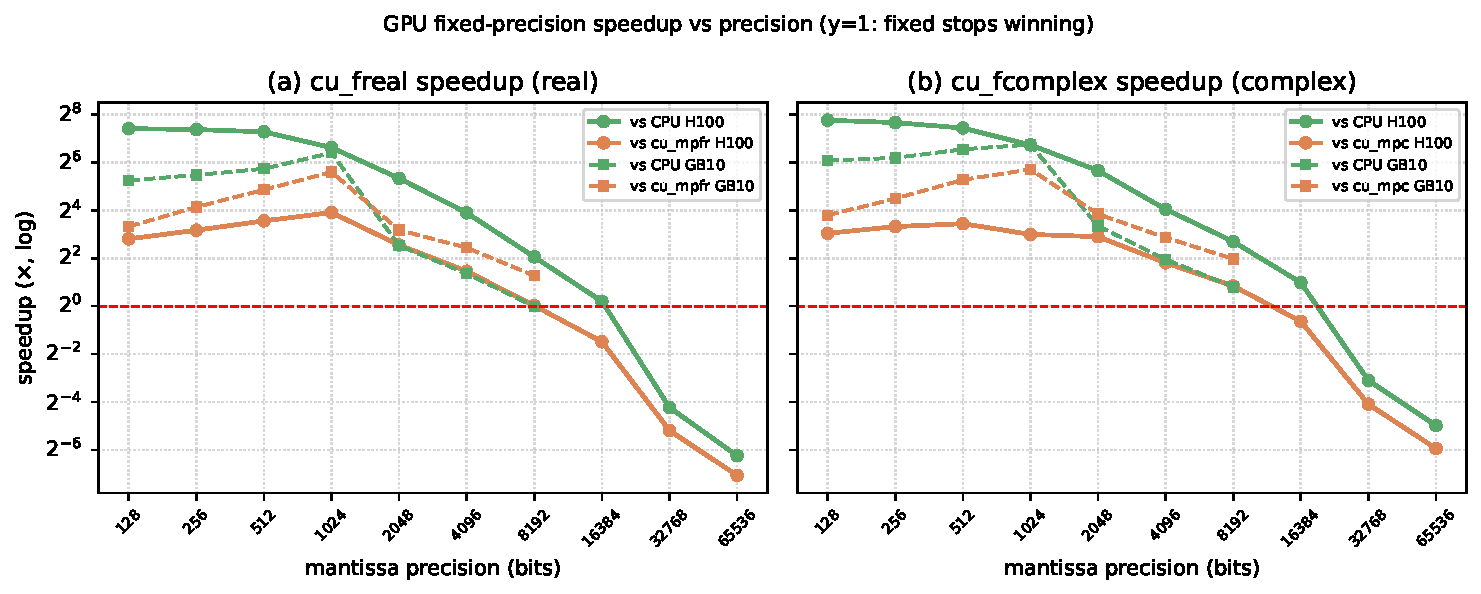
\includegraphics[width=0.98\textwidth]{figures/fig_speedup_gpu.pdf}
\caption{GPU 固定精度パスの速度比 vs 精度（両対数，$y=1$ がパリティ）。実線＝H100，破線＝GB10。
(a) 実数（対 CPU・対 cu\_mpfr），(b) 複素（対 CPU・対 cu\_mpc）。1024 ビットでピーク，
2048 ビットがスピル境界（knee），高精度で $y<1$ となり固定精度が負ける。}
\label{fig:speedup}
\end{figure}

H100 では大きなマシンがレイテンシをよく隠すため，第\ref{sec:platform}節の占有率の議論と
整合する 2 つの効果が現れる（表\ref{tab:bench3h100}）。第一に，\textbf{GPU ランタイム経路}
（\code{cu\_mpfr}/\code{cu\_mpc}）は\textbf{全精度で H100 が GB10 より約 2--5$\times$ 速い}
（例：1024 ビット実数で 0.120\,ms 対 GB10 の 0.388\,ms）。第二に，H100 の
\textbf{固定精度スピル境界（2048 ビット）ははるかに緩やか}で，\code{cu\_freal} は
1024$\to$2048 ビットで $\sim$2.75$\times$（0.008$\to$0.022\,ms）しか上がらない
（GB10 は $\sim$7$\times$，0.008$\to$0.056\,ms）。これは H100 の大きなレジスタファイルと
ローカルメモリ帯域がレジスタ$\to$ローカルのスピルを緩和するためである。

\paragraph{全経路の交差（H100）}
ビット長をさらに伸ばすと固定精度の優位は完全に消える。実数では \code{cu\_freal} が
\textbf{8192 ビットで cu\_mpfr とパリティ}（0.430 対 0.436\,ms），\textbf{16384 ビットで
CPU とも交差}（2.477 対 2.847\,ms）し，以降は急激に最悪化する（32768 ビットで 64.6\,ms，
65536 ビットで 482\,ms）。これはスピルした schoolbook $O(n^2)$ がローカルメモリを激しく
往復するためである。複素も同形で，\code{cu\_fcomplex} は 16384 ビットで cu\_mpc と，
32768 ビット手前で CPU と交差する。一方\textbf{GPU ランタイム経路は 65536 ビットでも CPU より速く}
（実数 3.6 対 6.4\,ms，複素 31.4 対 60.9\,ms），高精度では固定精度ではなくランタイム
（あるいは劣二次乗算を持つ CPU）が適することを示す。全スイープ点でホストとビット一致（\code{rel}=0）。

\begin{table}[h]
\centering
\caption{H100 での精度スイープ（AXPY，N=4096，全ビット一致）。GB10 は本機で再取得できないため
8192 ビットまでの表\ref{tab:bench3}を参照。時間は ms（8 回平均）。}
\label{tab:bench3h100}
\footnotesize
\begin{tabular}{rrrr@{\hskip 1.5em}rrr}
\toprule
 & \multicolumn{3}{c}{実数（MPFR）} & \multicolumn{3}{c}{複素（MPC）}\\
\cmidrule(r){2-4}\cmidrule(l){5-7}
ビット & \code{cu\_freal} & \code{cu\_mpfr} & CPU & \code{cu\_fcplx} & \code{cu\_mpc} & CPU \\
\midrule
128   & 0.004   & 0.028 & 0.681 & 0.009    & 0.074  & 1.955 \\
256   & 0.004   & 0.036 & 0.663 & 0.010    & 0.100  & 2.029 \\
512   & 0.005   & 0.059 & 0.776 & 0.015    & 0.163  & 2.595 \\
1024  & 0.008   & 0.120 & 0.786 & 0.044    & 0.351  & 4.670 \\
2048  & 0.022   & 0.129 & 0.888 & 0.125    & 0.932  & 6.309 \\
4096  & 0.083   & 0.228 & 1.235 & 0.509    & 1.785  & 8.403 \\
8192  & 0.430   & 0.436 & 1.787 & 2.025    & 3.626  & 13.105 \\
16384 & 2.477   & 0.884 & 2.847 & 11.693   & 7.529  & 23.115 \\
32768 & 64.635  & 1.769 & 3.443 & 263.499  & 15.429 & 30.636 \\
65536 & 482.420 & 3.601 & 6.375 & 1929.433 & 31.360 & 60.912 \\
\bottomrule
\end{tabular}\\[2pt]
\footnotesize 太字相当の転換点：実数は 8192 ビットで \code{cu\_freal}$\approx$\code{cu\_mpfr}，
16384 ビットで \code{cu\_freal}$>$CPU。複素は 16384 ビットで \code{cu\_fcplx}$\approx$\code{cu\_mpc}。
\end{table}

\subsection{CPU 上での固定精度パス}

\code{cu\_freal}/\code{cu\_fcomplex} はヘッダオンリーで，ホストでは \code{\_\_int128} を
用いて g++ のみでコンパイル・実行できる。CPU 単体（1 スレッド）で
システム MPFR/MPC と比較すると，\textbf{低精度でのみ速い}（表\ref{tab:cpu}）。
\code{cu\_freal} の乗算は schoolbook $O(n^2)$ だが GMP/MPFR は劣二次
（Karatsuba/Toom/FFT）であり，GPU で勝てたのはレジスタ常駐と大量並列で $O(n^2)$ を
隠せたからである。CPU 単スレッドにはその利点が無いため，約 512 ビットを超えると算法差がそのまま現れる。

\begin{table}[h]
\centering
\caption{CPU 単体での固定精度 vs システム MPFR/MPC（AXPY，N=4096，1 スレッド，速度比 $>1$ で固定精度が速い）}
\label{tab:cpu}
\begin{tabular}{rrr}
\toprule
ビット & freal/MPFR & fcplx/MPC \\
\midrule
128  & \textbf{1.28$\times$} & \textbf{1.79$\times$} \\
256  & \textbf{1.23$\times$} & \textbf{1.48$\times$} \\
512  & 1.03$\times$ & 0.99$\times$ \\
1024 & 0.71$\times$ & 0.67$\times$ \\
2048 & 0.09$\times$ & 0.17$\times$ \\
4096 & 0.03$\times$ & 0.06$\times$ \\
8192 & 0.01$\times$ & 0.03$\times$ \\
\bottomrule
\end{tabular}
\end{table}

\begin{figure}[h]
\centering
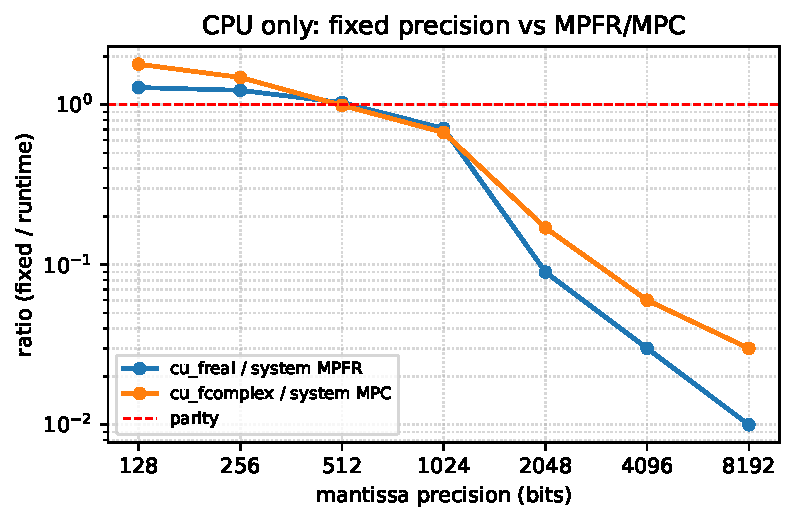
\includegraphics[width=0.82\textwidth]{figures/fig_cpu_crossover.pdf}
\caption{CPU 単体での固定精度 vs MPFR/MPC の比（縦軸対数，$y=1$ がパリティ）。
固定精度が上回るのは 128--256 ビットのみで，高精度では劣二次乗算を持つ MPFR/MPC が勝つ。}
\label{fig:cpu}
\end{figure}

\subsection{考察}

GPU では固定精度レジスタ常駐パスが\textbf{$\sim$1024 ビットまで圧勝}し
（CPU 比最大 $\sim$83$\times$，cu\_mpfr-GPU 比 $\sim$142$\times$），
2048 ビットでスピル境界（knee）を迎え，8192 ビットで CPU と同等になる。
一方 CPU 単体では同パスは 128--256 ビットでのみ MPFR/MPC を上回る。
すなわち固定精度 schoolbook の優位は\textbf{(i) GPU の並列性，(ii) 低〜中精度}に限られ，
高精度・CPU では劣二次乗算を備えた MPFR/MPC が適する。

\subsection{クロスプラットフォーム比較：GB10 vs H100（総括）}
\label{sec:platform}

最後に，本節で個別に併記してきた結果を 2 つの GPU の観点から総括する。
ランタイム精度の 6 デモ（実・複素 AXPY，行列ベクトル積，行列積）は同一ソース・
同一問題サイズ・1024 ビットで両機で実行され，全てビット一致である。2 台のホスト CPU が
異なる（GB10 の Grace ARM と H100 機の x86）ため，\textbf{GPU 時間 [ms]} が
ハードウェア同士の公平な指標であり，GPU vs CPU 速度比は参考として併記する
（表\ref{tab:platform}・図\ref{fig:platform}）。

\begin{table}[h]
\centering
\caption{GB10 vs H100，ランタイム精度デモ（1024 ビット，全ビット一致）。
比は GB10/H100 の GPU 時間（$>1$ で H100 が高速）。}
\label{tab:platform}
\begin{tabular}{lrrrr}
\toprule
デモ & $N$ & GB10 GPU & H100 GPU & H100/GB10 \\
\midrule
AXPY MPFR    & 16384 & 1.17\,ms  & 0.295\,ms & \textbf{3.97$\times$} \\
AXPY MPC     & 16384 & 4.81\,ms  & 1.037\,ms & \textbf{4.64$\times$} \\
行列ベクトル積 MPFR & 256 & 11.3\,ms & 15.80\,ms & 0.72$\times$ \\
行列ベクトル積 MPC  & 128 & 24.4\,ms & 29.68\,ms & 0.82$\times$ \\
行列積 MPFR  & 96    & 23.0\,ms  & 12.00\,ms & \textbf{1.92$\times$} \\
行列積 MPC   & 64    & 27.9\,ms  & 15.63\,ms & \textbf{1.79$\times$} \\
\bottomrule
\end{tabular}
\end{table}

\begin{figure}[h]
\centering
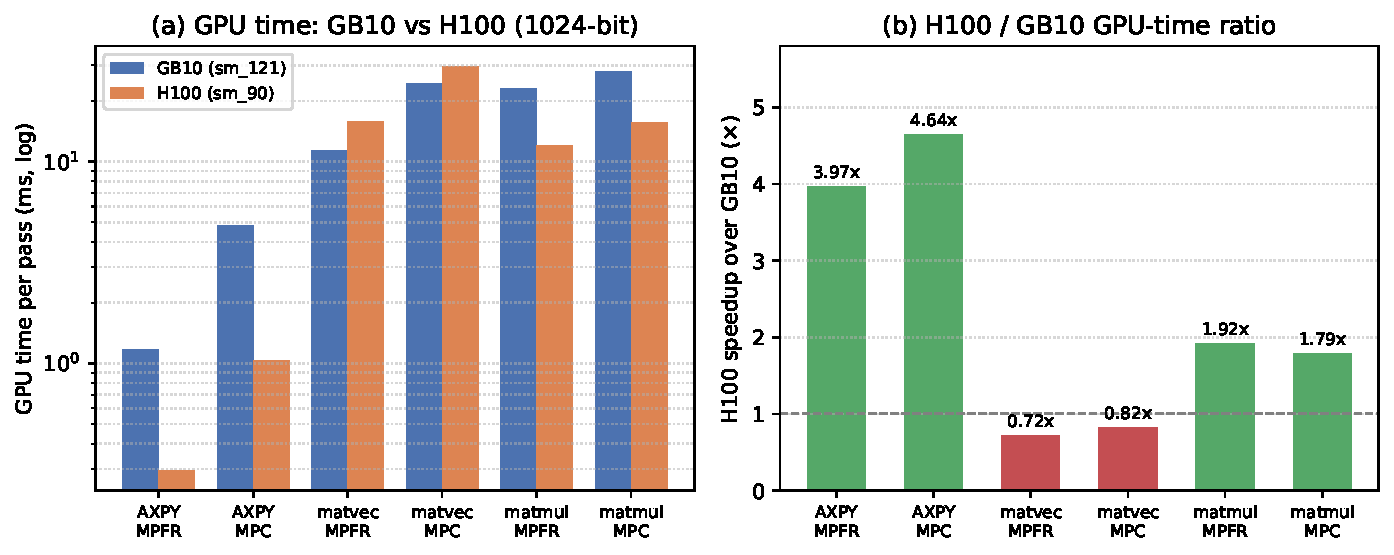
\includegraphics[width=0.98\textwidth]{figures/fig_gb10_vs_h100.pdf}
\caption{GB10 vs H100。(a) パスあたり GPU 時間（対数軸），(b) H100 の GB10 比速度
（$y=1$ がパリティ）。H100 は高並列カーネルで勝ち，小 $N$ の行列ベクトル積で負ける。}
\label{fig:platform}
\end{figure}

この傾向は占有率（occupancy）で一貫して説明できる。H100 は\textbf{高並列}カーネル
---AXPY（16384 要素のメモリバンド幅律速で $\sim$4$\times$）と行列積
（デバイスを飽和させる $O(N^2)$ グリッドで $\sim$1.8--1.9$\times$）---で，132 基の SM と
HBM3 バンド幅を活かして圧倒する。一方，行列ベクトル積では\textbf{負ける}
（0.72--0.82$\times$）：出力 1 行あたり 1 スレッドで $N=128$--256 ゆえ常駐スレッドは
高々 $\sim$128--256 にとどまり，起動が\textbf{占有率不足}となって 1 本の長い多倍長内積の
シングルスレッドレイテンシ律速となる。この領域では新しい GB10 コア（\code{sm\_121}，
高クロック）が速い。図\ref{fig:platspeedup} に 2 機の GPU vs CPU 速度比を並べて示す。

\begin{figure}[h]
\centering
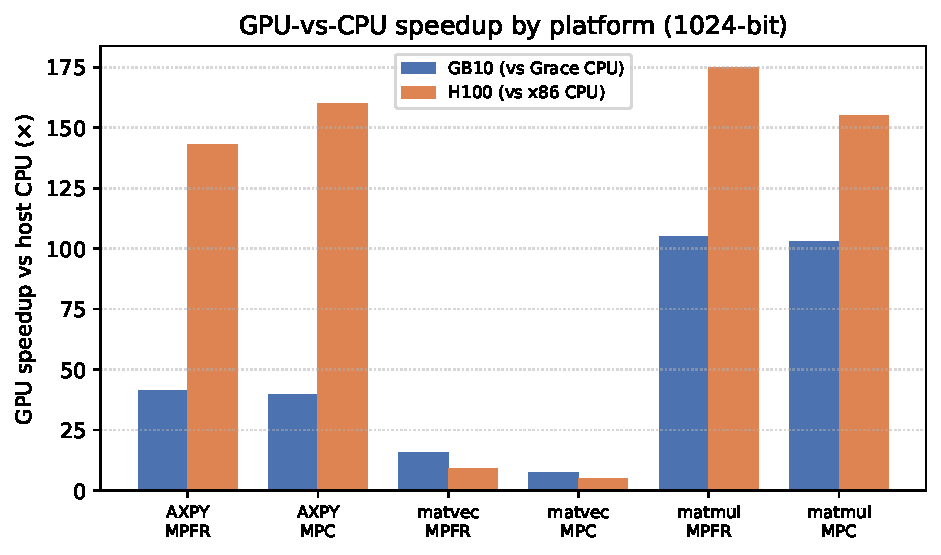
\includegraphics[width=0.7\textwidth]{figures/fig_platform_speedup.pdf}
\caption{プラットフォーム別の GPU vs CPU 速度比（各 GPU は自ホスト CPU 基準），1024 ビット。
H100 の高い AXPY/行列積速度比は，速い GPU と異なる（x86）ホスト基準の双方を反映する。}
\label{fig:platspeedup}
\end{figure}

\textbf{初等関数}（表\ref{tab:elemh100}・図\ref{fig:elemh100}）も同じ構図を示す：
$N=4096$ の関数評価はデバイスを十分に埋めるため両機で高速で，H100 は関数別に
\textbf{43--217$\times$}（対自ホスト x86），GB10 は \textbf{42--77$\times$}（MPFR）/
\textbf{22--63$\times$}（MPC，対 Grace ARM）に分布する。速度比は各々自ホスト基準ゆえ
直接比較はできないが，両機とも軽量カーネル（\code{sqrt}・\code{cbrt}・\code{sqr}）で上端，
多段 AGM の重いカーネル（\code{log}・複素 \code{asin}/\code{acos}）で下端という同形である。

\textbf{精度スイープ}（第\ref{sec:sweep}節）でも同じ占有率効果が一貫する：H100 は $N=4096$ で
レイテンシをよく隠すためランタイム経路が全精度で約 2--5$\times$ 速く，固定精度のスピル境界
（2048 ビット）も緩やかであった（GB10 $\sim$7$\times$ に対し H100 $\sim$2.75$\times$）。

要するに H100 は\textbf{埋めるだけの並列性がある時}（高並列 AXPY・行列積・初等関数・$N$ の大きい
スイープ）に優れ，GB10 は\textbf{レイテンシ律速の小 $N$ 領域}（行列ベクトル積）で競争力を持つ。

%======================================================================
\section{まとめと今後}
\label{sec:conclusion}

GMP(mini-gmp)/MPFR/MPC を，再実行可能な変換スクリプトにより\textbf{忠実に}
CUDA カーネル内へ移植し，実数 MPFR・複素 MPC の AXPY を CPU とビット一致のまま
約 40 倍高速化した。移植の核心は，コンパイル可能化（NORETURN/NO\_ASM/realloc/
\_Complex 等），デバイス実行可能化（RODATA/managed グローバル/確保経路/定数キャッシュ），
そして \code{mpfr\_div} のデバイス誤コンパイルに対する \code{mpz} ベース代替であった。
さらにスタック上限・アリーナ・並列度の調整，cu\_ 名前空間と umbrella による共存を整えた。

加えて，コンパイル時固定精度のレジスタ常駐型 \code{cu\_freal<PB>}/\code{cu\_fcomplex<PB>}
と固定精度初等関数を新設した。これらは GPU の低〜中精度で MPFR/MPC を桁違いに上回り，
精度スイープにより\textbf{2048 ビットがスピル境界，8192 ビットで CPU 同等}という
クロスオーバーを定量化した。さらに GB10 と H100 NVL のクロスプラットフォーム比較により，
ランタイム精度カーネルが\textbf{占有率律速}であることを示した：並列性が 132 基の SM を
埋められる AXPY（$\sim$4$\times$）・行列積（$\sim$1.8--1.9$\times$）では H100 が高速だが，
小 $N$ の行列ベクトル積はレイテンシ律速のままで GB10 がわずかに優る。

今後の課題は，MPFR/MPC の特殊関数（gamma, zeta, erf, Bessel 等）の固定精度実装，
高精度域のレジスタ圧・コンパイル時間の削減，固定精度向けの劣二次乗算
（Karatsuba 等）の導入，そして per-thread の指数・フラグ状態による完全な競合排除である。

\bigskip
\noindent\textbf{再現方法}：\code{./configure \&\& make}；\code{make check}（minigmp/mpfr/mpc/trans の
ビット一致），\code{make demos}/\code{matrix}/\code{bench}（性能），
\code{make sample-fixed}/\code{check-fixed}/\code{check-fmath}/\code{bench3}（固定精度）。
CPU 参照ターゲット（\code{bench3}・\code{coexist}・\code{cputest}・\code{cpubench}）は
システムの GMP/MPFR/MPC を要する。非標準のプレフィックスにある場合は
\code{./configure --with-mp-prefix=DIR}（例：\code{\textasciitilde/local}）を指定すると，
その \code{include}/\code{lib}（rpath 付き）がビルドに加わる。対象 GPU は
\code{--with-cuda-arch=ARCH}（既定 \code{sm\_90}；GB10 の測定は \code{sm\_121}）で選ぶ。
詳細はユーザマニュアル \code{doc/manual.ja.md}（日本語）/ \code{doc/manual.md}（英語）を参照。

\end{document}
